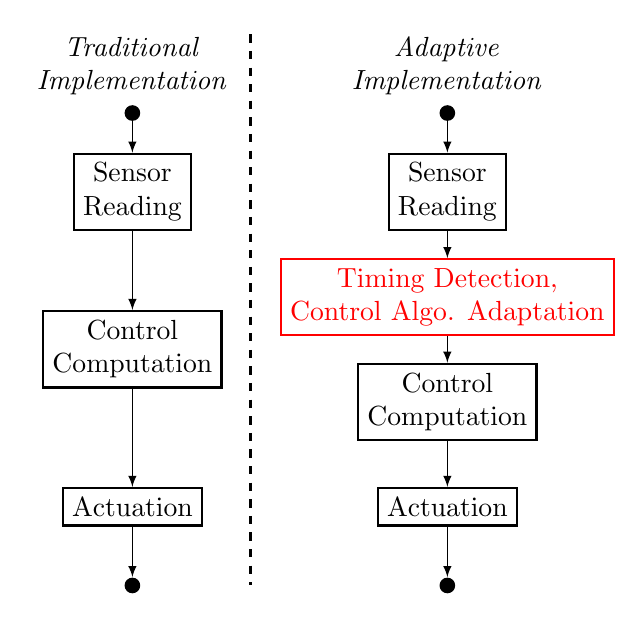
\begin{tikzpicture}
\tikzstyle{block} = [draw, thick, align=center]
\tikzstyle{io-dot} = [circle, fill, inner sep=2pt]

%%% NOMINAL %%%

\node[align=center] ()   at (-2,5.6) {\textit{Traditional}\\\textit{Implementation}};
\node[io-dot](in-nom)    at (-2, 5) {};
\node[block] (sense-nom) at (-2, 4) {Sensor\\Reading};
\node[block] (ctrl-nom)  at (-2, 2) {Control\\Computation};
\node[block] (act-nom)   at (-2, 0) {Actuation};
\node[io-dot](out-nom)   at (-2,-1) {};

\draw[-latex] (in-nom)    to (sense-nom);
\draw[-latex] (sense-nom) to (ctrl-nom);
\draw[-latex] (ctrl-nom)  to (act-nom);
\draw[-latex] (act-nom)   to (out-nom);

%%% INCREASE RUNTIME %%%

\node[align=center] ()   at ( 2,5.6) {\textit{Adaptive}\\\textit{Implementation}};
\node[io-dot](in-cod)    at ( 2, 5) {};
\node[block] (sense-cod) at ( 2, 4) {Sensor\\Reading};
\node[block,red] (tim-cod)   at ( 2, 2.66) {Timing Detection,\\Control Algo. Adaptation};
%\node[align=center, rotate=90] at ( 5, 2.66) {\textit{Perform Optimization (MPC)}\\\textit{re-Computing the controller}};
\node[block] (ctrl-cod)  at ( 2, 1.33) {Control\\Computation};
\node[block] (act-cod)   at ( 2, 0) {Actuation};
\node[io-dot](out-cod)   at ( 2,-1) {};

\draw[-latex] (in-cod)    to (sense-cod);
\draw[-latex] (sense-cod) to (tim-cod);
\draw[-latex] (tim-cod)   to (ctrl-cod);
\draw[-latex] (ctrl-cod)  to (act-cod);
\draw[-latex] (act-cod)   to (out-cod);

\draw[dashed, thick] (-.5,6) to (-.5,-1);

\end{tikzpicture}
